
\subsection*{Data augmentation}

Many trials in the dataset reveal a tendency from the participants to concentrate strokes to parts of the sketch. For example, many participants attended to the wheels of a car or the beak of the bird when trying to communicate their particular image, leaving remaining pieces of the image blank or oversimplified. This behavior seems particular useful in close-contexts, where global structure between target and distractor images is hard to distinguish whereas local structure hold more obvious differences. To mimic this behavior from a computational model, and to increase the size of the dataset, we propose the following augmentation technique: given a rendered image, choose a subset of the image and replace the rest of the pixels with a default background color (RGB: 127, 127, 127). This has the effect of obscuring the majority of the image, allowing the visual encoder module to attend to particular fragments. In practice, given an image of size 256x256, we first find a bounding box around the non-background color pixels. Starting from the top-left corner of the bounding box to the bottom-right, we choose continguous 75x75 pixel subsets of the image. This produces between 4 and 32 subsets per image, with an average of 27. The original image remains in the dataset. Using this procedure, we augment the dataset from 3072 to 24576 images. For each image, the corresponding sketch is left untouched. Figure TODO shows examples augmented images.

\begin{figure}[h!]
    \centering
    \subfloat[Bird]{
        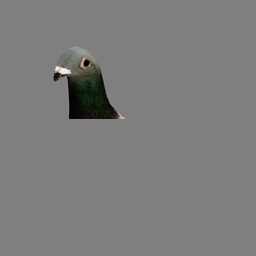
\includegraphics[width=0.20\linewidth]{figures/bird_crop_example.png}
    }
    \subfloat[Chair]{
        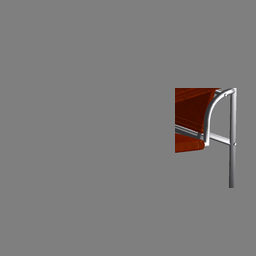
\includegraphics[width=0.20\linewidth]{figures/chair_crop_example.png}
    }
    \subfloat[Dog]{
        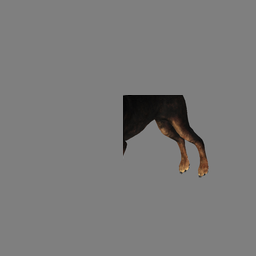
\includegraphics[width=0.20\linewidth]{figures/dog_crop_example.png}
    }
    \subfloat[Car]{
        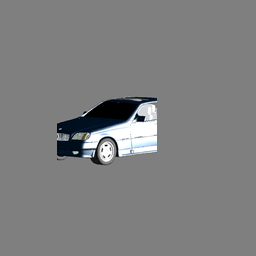
\includegraphics[width=0.20\linewidth]{figures/car_crop_example.png}
    }
    \caption{Examples of data augmentation on rendered images. For each image, everything except a section is hidden. By doing so, we introduce an \emph{attention} mechanism where the model can learn to associate sketches to particular details in the rendered image.}
    \label{fig:augment_example}
\end{figure}
